% Evaluation paper: audit of the deployed data-matching judge (FINAL_v2).
% Every number is read from FINAL_v2/v2_gridsearch/REPORT.md (generated 2026-09-27 13:12) and output/.
% Figures: FINAL_v2/paper/figures/.  Compile from FINAL_v2/paper/ with pdflatex.
\documentclass[11pt]{article}
\usepackage[margin=1in]{geometry}
\usepackage{booktabs,graphicx,longtable,tabularx,array,caption,subcaption,amsmath,hyperref,enumitem,xcolor}
\usepackage[T1]{fontenc}
\usepackage{lmodern}
\captionsetup{font=small,labelfont=bf}
\setlist{nosep,leftmargin=*}
\newcolumntype{L}{>{\raggedright\arraybackslash}X}
\graphicspath{{figures/}}
\emergencystretch=1.5em
\hypersetup{colorlinks=true,linkcolor=blue!60!black,citecolor=blue!60!black,urlcolor=blue!60!black}

\title{Auditing a Deployed LLM Judge for Data Matching:\\Is Any Weighting of Its Ingredients Better Than the One It Ships With?}
\author{}
\date{2026}

\begin{document}
\maketitle

% =====================================================================
\section{Related work: other processes and inspirations}
% (user text, unchanged)
\begin{itemize}
\item s
\end{itemize}

\subsection*{Lit review checks}
\begin{description}[style=unboxed,leftmargin=0pt,itemsep=4pt]
\item[] \textbf{Pairwise-comparison leaderboards: Chatbot Arena (Chiang et al., 2024)}\\
Did: Bradley--Terry strengths from millions of human pairwise votes with bootstrap confidence intervals. Took: Bradley--Terry as the headline pooling rule and item-level bootstrap rank intervals. Changed: the pairwise ``votes'' are item-level score comparisons from a gold-based judge, so the judge itself is audited; the leaderboard is reported under several pooling rules rather than one.
\item[] \textbf{Rank aggregation for benchmarks: Colombo et al. (2022); Kemeny (1959); Borda}\\
Did: argued for Kemeny / Borda consensus over mean scores when aggregating NLP benchmarks, because means are sensitive to scale and outliers. Took: Borda inside the objective (cheap, robust), Kemeny and Copeland as checks, and the Kemeny cost as a saved parameter. Changed: we quantify how much the choice of rule changes the top order on the same scores.
\item[] \textbf{Holistic, native-metric evaluation: HELM (Liang et al., 2022)}\\
Did: per-scenario native metrics, mean win rate across scenarios, no composite. Took: the idea that each dataset keeps its own metric as a baseline column (our ``native'' rule and $\tau$-to-native). Changed: we study the composite because the deployed judge uses one, and show its weights do not matter on this suite.
\item[] \textbf{Few-item evaluation and IRT: tinyBenchmarks (Polo et al., 2024)}\\
Did: showed $\sim$100 well-chosen items reproduce full-benchmark rankings, using item-response theory. Took: 100 items per dataset as the design target and a Rasch ability view in the sibling v3 pipeline. Changed: our items are stratified by task structure rather than selected by IRT informativeness; we report the attainable precision directly through item bootstraps.
\item[] \textbf{Benchmark agreement and reliability: Perlitz et al. (2024, BenchBench); Boubdir et al. (2023, Elo Uncovered)}\\
Did: measured how much benchmarks agree about model rankings and how reliable Elo-style ratings are (transitivity, sensitivity to the order and set of comparisons). Took: Kendall's $W$ among datasets, $\tau$ between pooling rules, and the stability of rankings under resampling as first-class outputs. Changed: applied to datasets inside one suite rather than to whole benchmarks.
\item[] \textbf{Comparing systems over many datasets: Dem\v{s}ar (2006); Garc\'ia \& Herrera (2008)}\\
Did: established the Friedman test with Nemenyi or Holm post-hoc as the correct way to compare classifiers across datasets. Took: exactly that battery, plus the Iman--Davenport correction. Changed: added per-item paired tests within datasets (Koehn, 2004; Dror et al., 2018) because we have item-level scores, which the classic setting does not.
\item[] \textbf{Selection bias and nested validation: Cawley \& Talbot (2010); Varma \& Simon (2006)}\\
Did: showed that choosing a model or hyper-parameter on the same data used to report its performance biases the report upward, and that nested cross-validation removes the bias. Took: the nested item bootstrap (select in-bag, score out-of-bag) and the optimism gap as a reported quantity. Changed: applied to weight search for a judge, and extended with the plateau, which turns ``the best weighting'' into a set.
\item[] \textbf{Metric meta-evaluation: Mathur et al. (2020); Kocmi et al. (2021); SummEval (Fabbri et al., 2021)}\\
Did: validated automatic metrics against human judgements and showed that correlations are driven by outlier systems and that metric choice changes decisions. Took: the principle that a judge must be validated against a quality signal external to the systems it ranks, the outlier diagnostics, and the design of the human-labelling protocol (two labellers, adjudication, agreement statistics). Changed: our external signal is synthetic (controlled perturbations of gold answers) until human labels exist; we keep agreement and correctness as separate axes. (Similar to Chatbot reasoning.)
\item[] \textbf{Behavioural testing with controlled perturbations: CheckList (Ribeiro et al., 2020)}\\
Did: tested NLP models with templated, typed perturbations whose expected outcome is known. Took: the operator idea for the anchors: every synthetic answer has a type (alias, unit change, magnitude error, hedge, \dots) and a known utility. Changed: the perturbations are applied to gold answers to test the judge, not to inputs to test the model (to check that small discrepancies have similar output).
\item[] \textbf{LLM judges and their validation: MT-Bench (Zheng et al., 2023); JudgeBench (Tan et al., 2024); G-Eval (Liu et al., 2023)}\\
Did: used LLMs as judges and measured their agreement with humans; built benchmarks of hard judging cases. Took: the framing that any judge is a model of quality and needs validation; the refusal and hedge handling. Changed: our judge is a formula over lexical metrics, which is cheaper, deterministic and auditable but blind to semantics (prompt structure impact, etc.); we state that trade-off rather than mixing in an LLM judge.
\item[] \textbf{Search designs: McKay, Beckman \& Conover (1979); Bergstra \& Bengio (2012); Hickernell (1998)}\\
Did: Latin hypercube sampling for even coverage; random search beating grids when few dimensions matter; discrepancy as a coverage measure. Took: three designs (uniform lattice, Dirichlet-snapped, Latin hypercube on the simplex via exponential spacings) with centred $L_2$ discrepancy and nearest-neighbour distances. Changed: for four weights the exhaustive grid replaces all of them; the designs remain for the larger sibling searches and as evidence that sampling would have sufficed.
\item[] \textbf{Variance in benchmarks: Bouthillier et al. (2021); Card et al. (2020); Renze \& Guven (2024)}\\
Did: decomposed benchmark variance into data sampling, initialisation and other sources; showed most NLP test sets lack power; found temperature in 0--1 does not change problem-solving accuracy. Took: item bootstraps everywhere, 100 items per dataset, temperature 0 as a reproducibility choice with a planned repeat subset. Changed: documented which providers refuse temperature control and recorded the decoding per answer.
\item[] \textbf{Class imbalance in matching benchmarks: Papadakis et al. (2024)}\\
Did: re-evaluated entity-matching benchmarks and showed that the usual balanced or easy splits overstate matcher quality; released re-balanced sets (Dn1--Dn8). Took: the Dn sets in the suite at their real ratios, and the motivation for post-stratification. Changed: balanced pools are kept for calibration while official-ratio F1 is reported for comparability.
\item[] \textbf{Survey estimation: Horvitz \& Thompson (1952)}\\
Did: unbiased estimation of a population mean from a sample with known inclusion probabilities. Took: post-stratification weights (official share / sample share) and the weighted bootstrap. Changed: applied to benchmark items as a population, with the official split as the target.
\item[] \textbf{Leaderboard integrity: The Leaderboard Illusion (Singh et al., 2025)}\\
Did: documented how private testing and selective reporting distort a public leaderboard. Took: the discipline of reporting every candidate and every bootstrap draw, archiving replaced answers, and tagging re-asks. Changed: our selection effect is weight search rather than model submission, and the nested bootstrap is the counter-measure.
\item[] \textbf{Qualitative model differences: VibeCheck (Dunlap et al., 2024)}\\
Did: extracted and quantified qualitative traits that predict human preference. Took: the reminder that a lexical judge cannot see style, hedging or formatting quality; the hedge flag is our one concession. Changed: nothing adopted; cited as the complementary axis our evaluation does not cover.
\end{description}

% =====================================================================
\section{Experiment procedure}
% (user text, unchanged)
\begin{enumerate}
\item
\begin{itemize}
\item Gathered 100 most cited, relevant datasets in $\sim$220 top-cited papers relating to the field of data matching, according to the following criteria of relevance, adoption, generalisation, discriminative power, gold clarity, inclusivity, licence.
\item Kept top 30 most-cited datasets among the shortlisted collection of datasets, and accounted for inclusivity and redundancy of dataset types, with the following distribution:
\begin{itemize}
\item entity matching: 11, schema matching: 6, table QA: 11, financial documents: 3.
\item Pools of 150 items per dataset by seeded stratified sampling from the official split (strata: question type, sub-task, database, product category, or match label), with 100 fed to the model for output answers (except for two smaller datasets, which took total rows of 90 and 93).
\item Then balanced positive and negative pairs for prompts to a 50:50 ratio, excluding the Papadakis--Christen entity-matching datasets (which kept their imbalance ratio intentionally).
\end{itemize}
\end{itemize}
\item
\begin{itemize}
\item Scores a given prompt output ``answer'' in the following way:
\[ R = 0.35\,\mathrm{F1} + 0.35\,e^{-2.5\,|\text{relative numeric error}|} + 0.15\,\mathrm{Precision} + 0.15\,\mathrm{Recall}. \]
\item Decay, Precision, Recall calculated by comparing model prompt output to the ground-truth gold, per row data element.
\item Each gold in the ground-truth set is calculated via controlling for aliases (text-intensive answers), unit and percent occurrences, and words representing the scale of numbers.
\end{itemize}
\item The following models were tested, ensuring flagship models and competitive flash-model alternatives were chosen for all major LLM open-source and private models:
\begin{itemize}
\item Claude Opus 5, Claude Sonnet 5, GPT-5.5, GPT-5.4-mini, Gemini 3.8 Flash, Grok 4, DeepSeek-chat, DeepSeek-R1, gpt-oss-120b, Llama 3.3 70B (ten; Gemini 3.1 Pro col\-lected at 240 items a day and included once it reaches 90\,\% coverage).
\end{itemize}
\end{enumerate}

% =====================================================================
\section{Setup}
\label{sec:setup}

\subsection{Suite and pools}
\begin{itemize}
\item 31 datasets: 11 entity matching (EM), 6 schema matching (SM), 11 table question answering and understanding (TQA), 3 financial documents (FIN). Each adapter reads the official test or dev split and emits items with a question, a context (table, document, or record pair), a gold answer with aliases, a list gold where the answer is a set, an answer type (numeric / boolean / text / free-form) and the dataset's native metric.
\item Pools: 150 items per dataset by seeded stratified sampling (strata: question type, sub-task, database, product category, match label); 100 flagged for answering (OfficeQA Pro V2: all 90; Alaska schema: 93). The remaining 50 are a seeded reserve and are not used by any step. Total answered items: 3,083 per model.
\item Entity-matching pools are 50/50 match / non-match (Papadakis--Christen keeps its real 1.8\,\% match ratio). Schema matching is framed as one question per source column with a candidate list that always contains the gold. BIRD is graded on the executed result of the gold SQL, not on SQL text.
\item Official census: every dataset's official population is counted by the same strata, so that pool numbers can be re-weighted to the official split (Section~\ref{sec:setup:official}).
\end{itemize}

\subsection{Collecting answers}
\begin{itemize}
\item One prompt per item: context, question, and an answer-format line requesting \texttt{FINAL ANSWER: <answer>}.
\item Models: Claude Opus 5, Claude Sonnet 5, GPT-5.5, GPT-5.4-mini, Gemini 3.8 Flash, Grok 4, DeepSeek-chat, DeepSeek-R1, gpt-oss-120b (Together), Llama 3.3 70B (Together). Gemini 3.1 Pro is collected separately at 240 items a day by a scheduled GitHub Actions workflow and enters the study automatically at 90\,\% suite coverage.
\item Decoding: temperature 0 where the API accepts it (Gemini, Grok, DeepSeek, Llama, gpt-oss). Claude 5 reports the parameter deprecated and GPT-5.5 rejects any non-default value; those ran at provider defaults. Every cached row records which applied.
\item Output budget 700 tokens. A reply cut off for length with no final-answer line is re-asked at 2,500 tokens, then at 8,000. The trigger is mechanical (finish reason plus absence of the final line), never correctness. Originals are archived with a reason; replacement rows carry \texttt{attempt} = 2 or 3. Replies still unterminated at 8,000 tokens are scored as given (effectively failures).
\item Every answer is cached with tokens, latency, cost, finish reason and decoding; re-runs skip cached items. Cost: USD 161 for ten models (Claude Opus 5: USD 99).
\end{itemize}

\subsection{Scoring an answer}
\begin{itemize}
\item Extraction: the \texttt{FINAL ANSWER:} line; else a boxed expression; else the last short line of the reply.
\item Normalisation: Unicode NFKC, lower-case, canonical numbers (``1,577.00'' $\to$ ``1577'', ``(12.6)'' $\to$ ``$-$12.6''), currency symbols and punctuation removed, articles dropped, whitespace collapsed.
\item Units and scale: every number is parsed with sign, percent marker (\%, ``percent'', ``pp'') and scale word (thousand / million / billion / trillion and abbreviations). A parsed number exposes its equivalent readings (raw, scaled, $\div 100$ if marked percent, $\times 100$ if an unmarked fraction); the relative error between prediction and gold is the minimum over all pairs of readings. Real-unit conversions (km $\leftrightarrow$ miles) are not attempted.
\item Aliases: each item carries the primary gold plus acceptable alternatives supplied by the adapter (e.g.\ \emph{yes} $\equiv$ \emph{match} $\equiv$ 1; several legitimate target columns in schema matching; comma- and pipe-joined forms of list golds). Every component is computed against each alias and the best-scoring alias is kept. Booleans are canonicalised before comparison.
\item Components per answer: token F1, numeric decay $e^{-2.5\cdot\text{rel.\ err}}$ (error clipped at 2; falls back to exact match for non-numeric golds), token precision, token recall; also exact match, numeric tolerance (1\,\%), ROUGE-L, and a hedge flag (several distinct numeric candidates, ``A or B'', or an enumeration of short candidates).
\item Native metric per dataset (baseline column): numeric tolerance for numeric golds, exact match for text and boolean golds, ROUGE-L for free-form (FeTaQA).
\item Composite under weighting $w$ on the simplex: $R_w = \sum_k w_k m_k$, $k \in \{$F1, decay, precision, recall$\}$. v1 is $w = (0.35, 0.35, 0.15, 0.15)$.
\item Dataset score of a model: mean $R_w$ over the items that every model answered. A model is in the study only if it covered $\ge 90\,\%$ of the suite; a dataset is used only with $\ge 20$ answered items.
\end{itemize}

\subsection{Evaluating a weighting}
\begin{enumerate}
\item \textbf{Agreement $J(w)$.} Rank the ten models inside each dataset under $w$; pool the 31 rankings by Borda; $J$ is the mean Kendall $\tau_b$ between each dataset's ranking and the pooled one. $J$ measures consistency between datasets, not correctness. Computed for all 1,771 weightings of the step-0.05 simplex lattice (v1, the four corners and the uniform mix are lattice points), and also under Kemeny, Copeland and Bradley--Terry pooling.
\item \textbf{Correctness $\rho(w)$.} 31,380 synthetic answers of known utility generated from the golds of the answered items by typed operators (identity, alias, unit variant, typo, rounding, magnitude error, sign flip, wrong value, partial list, superset, hedge, verbose, no answer, \dots). Reported: Spearman $\rho$ between $R_w$ and utility, AUC correct vs wrong, mean score of wrong answers, hedge gap; the $(J,\rho)$ Pareto front and its knee.
\item \textbf{Honest selection.} Nested item bootstrap ($B=1{,}000$): choose the best $w$ on in-bag items, score it out of bag. Reported: the optimism gap, the paired out-of-bag difference to v1 with a 95\,\% interval, and the plateau (weightings not significantly below the best, paired bootstrap $p>.05$) plus a practical plateau (within 0.02 of the best).
\item \textbf{Transfer.} Leave-one-dataset-out and leave-one-family-out: re-fit $w$ on the rest, measure $\tau$ of the held-out dataset's ranking to the pooled rest; per-family optima; sensitivity to one lattice step (0.05).
\item \textbf{Designs.} Uniform-lattice, Dirichlet-snapped and Latin-hypercube samples of 100 weightings, 20 seeds each, compared with the exhaustive optimum (regret, rank of the found best, centred $L_2$ discrepancy, minimum pairwise $L_1$).
\end{enumerate}

\subsection{From scores to a leaderboard}
\label{sec:setup:official}
\begin{itemize}
\item Rules reported: exact match only, v1, the five best by $J$, the best by $\rho$, the $(J,\rho)$ Pareto knee.
\item Pooling: Bradley--Terry strengths from item-level pairwise wins (MLE, ridge 0.01, standard errors from the observed information) as the headline; Borda, mean-$z$, Kemeny (with cost), Copeland, reciprocal-rank fusion and family-balanced $z$ as checks.
\item Uncertainty: 1,000 item bootstraps of the Borda and Bradley--Terry rankings (rank intervals, probability of first place), saved in full.
\item Significance: Friedman with the Iman--Davenport correction across datasets, Nemenyi critical difference, Holm-corrected pairwise Wilcoxon; paired permutation and Wilcoxon per dataset and model pair (Holm within dataset); Kendall's $W$ among datasets; majority-class baselines for boolean sets.
\item Official-split estimates: the same answers re-weighted by official stratum share / sample share (post-stratification) with a weighted item bootstrap; positive-class precision, recall and F1 at the official match ratio for the matching sets.
\item Diagnostics: pairwise $\tau$ between dataset rankings; floor, ceiling and self-stability flags per dataset.
\item Reporting: one script regenerates the report from the cached answers in minutes, so text and numbers cannot disagree.
\end{itemize}

% =====================================================================
\section{Methods / logic}
% (user placeholder, unchanged)
\begin{itemize}
\item s
\end{itemize}

% =====================================================================
\section{Results}
\label{sec:results}

All numbers are from the final run of 2026-09-27 (31 datasets $\times$ 10 models, 3,083 answered items per model). Table~\ref{tab:summary} gives the audit in one place; the subsections that follow give one figure or table per row.

\begin{table}[htbp]
\centering\small
\caption{Audit summary. $J$ = agreement objective (mean Kendall $\tau_b$ of each dataset's model ranking to the Borda pool); $\rho$ = Spearman correlation of the composite with known utility on 31,380 synthetic anchors.}
\label{tab:summary}
\begin{tabularx}{\textwidth}{>{\bfseries}p{0.30\textwidth} L}
\toprule
Exhaustive grid & 1,771 weightings (step 0.05); best decay .70 / recall .30, $J=0.421$; v1 $J=0.404$ (rank 1,483 of 1,771) \\
$J$ over the lattice & median 0.409, 90th percentile 0.415, 99th percentile 0.418: a flat landscape \\
Plateau (paired bootstrap $p>.05$ vs best) & 1,765 of 1,771 (v1 inside, $p=0.66$); practical plateau within 0.02: 1,720 \\
Nested selection ($B=1{,}000$) & in-bag $J$ of the selected weighting 0.380, out-of-bag 0.331 (optimism gap 0.049); v1 out-of-bag 0.339 \\
Selected vs v1, out of bag & $-0.008$, 95\,\% CI $[-0.039,\,+0.013]$, $p=0.72$; 608 distinct weightings selected across resamples \\
Sampled designs (100 points, 20 seeds) & Dirichlet / LHS / uniform all reach $0.418\pm0.001$, regret $\le 0.005$: sampling would have sufficed \\
Objective under other pooling rules & Kemeny, Copeland and Bradley--Terry each pick a different ``best''; v1's rank swings from 393 to 1,506: rank is noise \\
Transfer (leave-one-dataset-out) & held-out $\tau$: LODO weights $+0.34$, full best $+0.39$, v1 $+0.37$ \\
Leave-one-family-out & v1 within 0.02 of the held-out-fitted weights on EM, SM, TQA; FIN favours precision-heavy weights ($+0.51$ vs $+0.43$) \\
Anchors (31,380 synthetic answers) & v1 $\rho=0.878$, best-$\rho$ weighting 0.883, best-$J$ weighting 0.845, exact match 0.828; AUC correct-vs-wrong 0.994 for every rule \\
$J$ vs $\rho$ across the lattice & $-0.34$ on this cache; $+0.38$ on the previous cache: unstable because $J$ is flat \\
Sensitivity & one 0.05 step moves $J$ by at most 0.007 around v1 and 0.005 around the best \\
Leaderboard & Friedman $p<0.001$ under every rule; Kendall's $W$ among datasets 0.26--0.28 \\
Significant pairs (Holm) & Opus, Sonnet, GPT-5.5, Gemini Flash, DeepSeek-chat, DeepSeek-R1, GPT-5.4-mini, Grok 4 all $>$ Llama 3.3 70B; Opus, Gemini Flash, GPT-5.5, Grok 4 $>$ gpt-oss-120b \\
First place & Bradley--Terry: Gemini 3.8 Flash under v1 and the calibrated rules ($P(\text{first})=0.99$), Opus under exact match; Borda: GPT-5.5 under v1, Opus under exact match and the top-5 rules \\
Official-split comparability & accuracy moves by $\le 0.09$ after post-stratification; positive-class F1 on the balanced pools overstates official-ratio F1 by up to 0.19 (Amazon--Google) \\
Datasets at ceiling & Valentine, WDC LSPC, WDC Products (means 0.98): flagged; still inside the objective \\
Cost & USD 161 total (Opus 99) \\
\bottomrule
\end{tabularx}
\end{table}

\subsection{The objective is flat}
Figure~\ref{fig:landscape} shows $J$ for all 1,771 weightings. The whole lattice spans 0.39--0.42. The best weighting (decay 0.70, recall 0.30) reaches 0.421 and v1 reaches 0.404; 1,482 weightings are nominally better than v1, but the entire spread is smaller than the bootstrap noise of a single weighting. No single weight has a slope worth acting on (Figure~\ref{fig:marginals}).

\begin{figure}[htbp]
\centering
\begin{subfigure}{0.48\textwidth}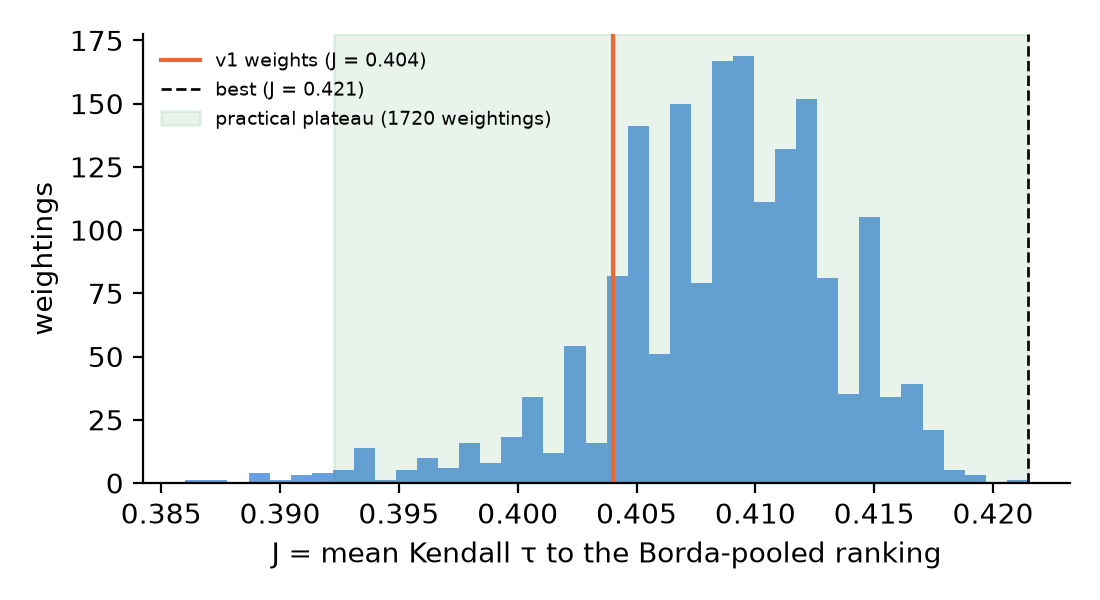
\includegraphics[width=\linewidth]{fig_j_histogram.png}\caption{Distribution of $J$ over the lattice with v1, the best and the plateau band.}\end{subfigure}\hfill
\begin{subfigure}{0.48\textwidth}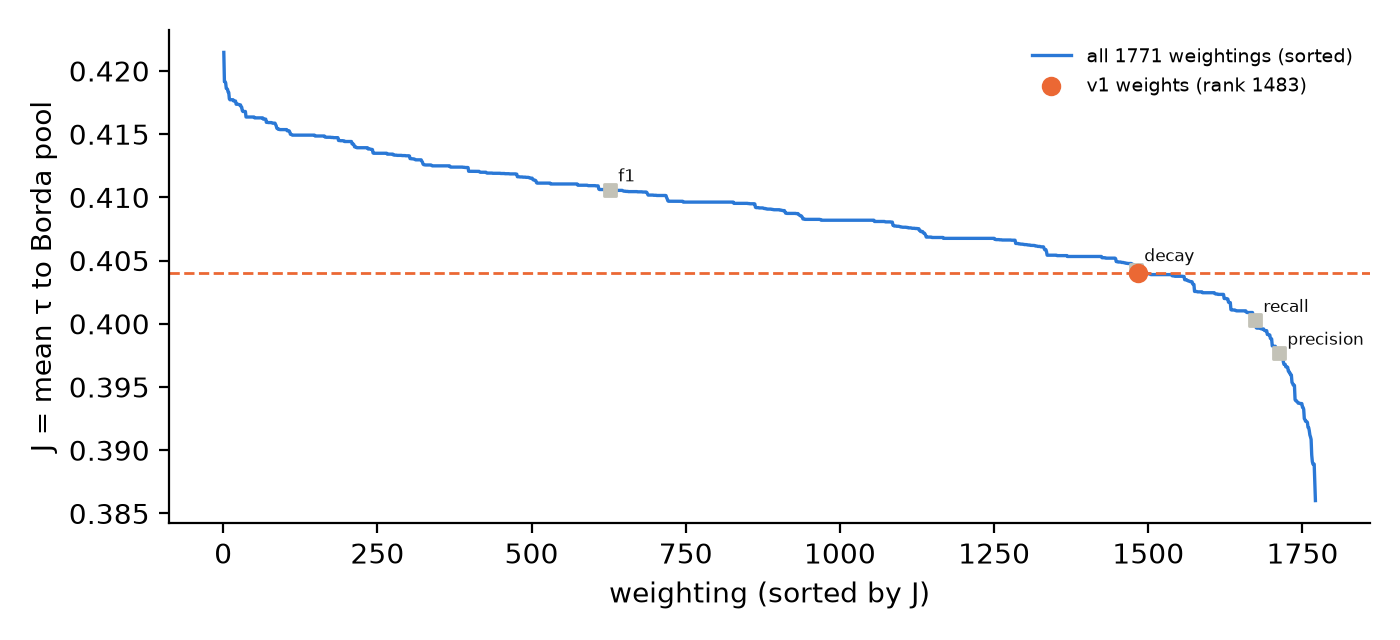
\includegraphics[width=\linewidth]{fig_landscape.png}\caption{Sorted $J$ with v1 and the four single-ingredient corners.}\end{subfigure}
\caption{The agreement landscape over all 1,771 step-0.05 weightings.}
\label{fig:landscape}
\end{figure}

\begin{figure}[htbp]
\centering
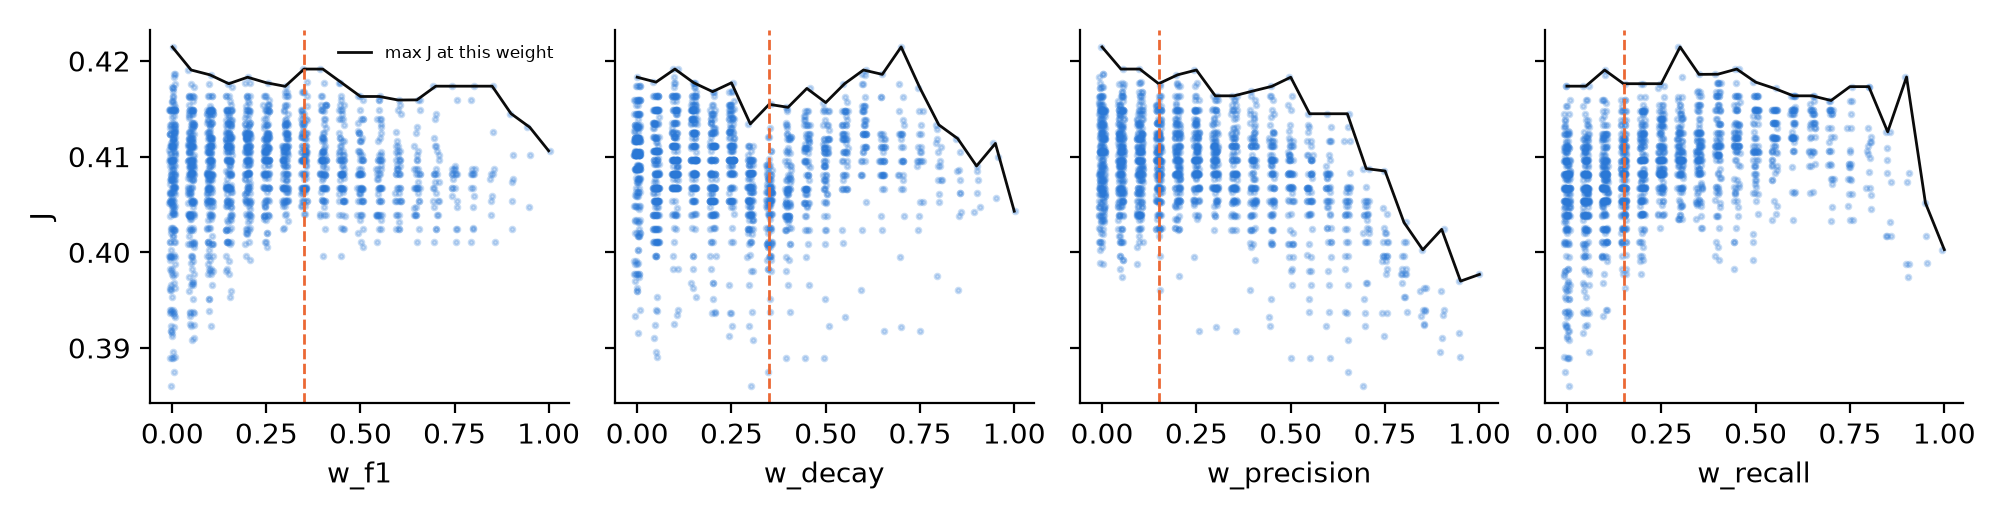
\includegraphics[width=0.95\textwidth]{fig_marginals.png}
\caption{$J$ against each of the four weights. Corners: F1 only 0.411, decay only 0.404, precision only 0.398, recall only 0.400; uniform 0.410.}
\label{fig:marginals}
\end{figure}

\subsection{The best weighting does not survive honest selection}
Figure~\ref{fig:nested} reports the nested item bootstrap. The weighting chosen on in-bag items scores 0.380 in bag but 0.331 out of bag (optimism gap 0.049), below v1's out-of-bag 0.339. The paired out-of-bag difference to v1 is $-0.008$ with a 95\,\% interval of $[-0.039, +0.013]$ ($p=0.72$); the selected weighting is ahead of v1 in 28\,\% of resamples, and 608 distinct weightings were selected across the 1,000 resamples. The plateau of weightings not significantly below the best contains 1,765 of 1,771 points and v1 is inside it ($p=0.66$).

\begin{figure}[htbp]
\centering
\begin{subfigure}{0.48\textwidth}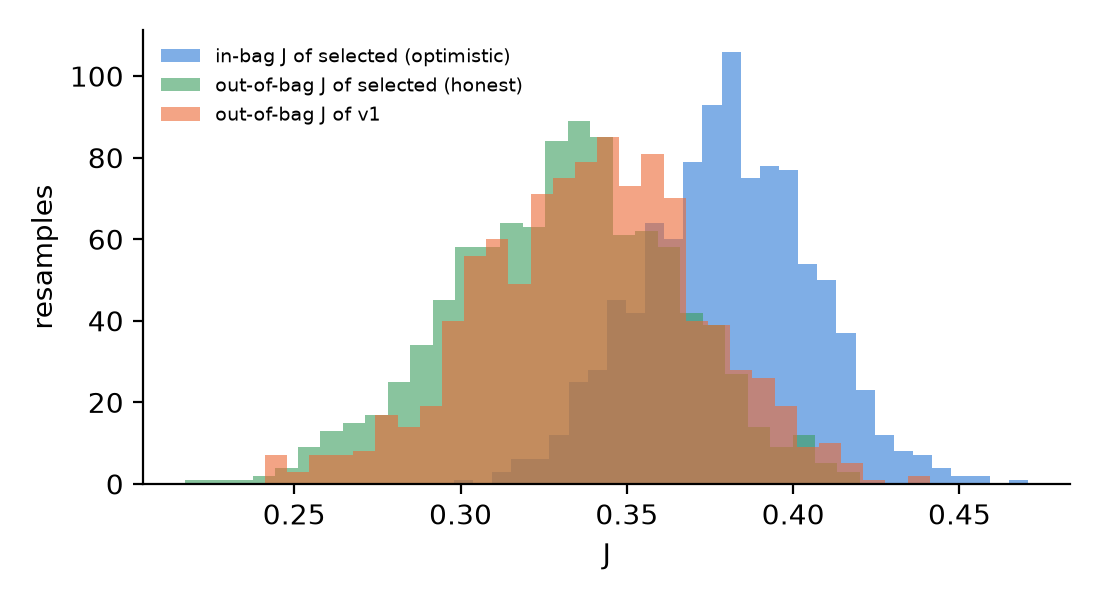
\includegraphics[width=\linewidth]{fig_nested.png}\caption{In-bag vs out-of-bag $J$ of the selected weighting against v1.}\end{subfigure}\hfill
\begin{subfigure}{0.48\textwidth}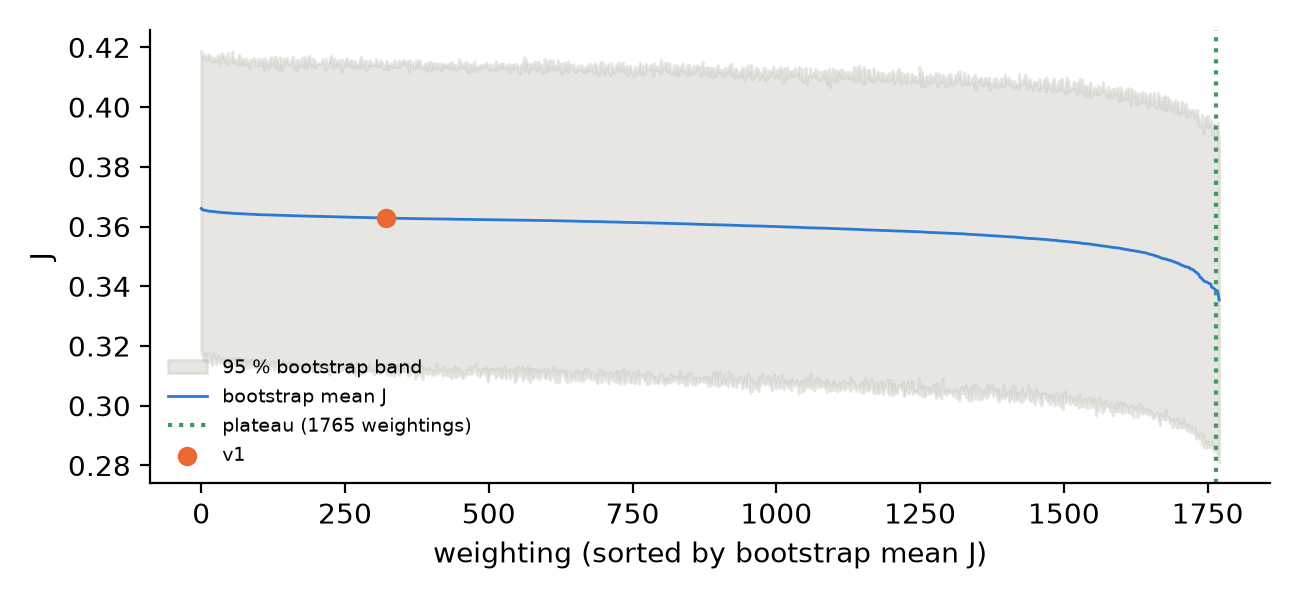
\includegraphics[width=\linewidth]{fig_plateau.png}\caption{Bootstrap band over sorted weightings; the plateau boundary.}\end{subfigure}
\caption{Honest selection: the optimism gap and the plateau.}
\label{fig:nested}
\end{figure}

\begin{table}[htbp]
\centering\scriptsize
\caption{Sampled designs at a budget of 100 weightings (20 seeds each) against the exhaustive optimum.}
\label{tab:designs}
\begin{tabularx}{\textwidth}{l>{\centering\arraybackslash}X>{\centering\arraybackslash}X>{\centering\arraybackslash}X>{\centering\arraybackslash}X>{\centering\arraybackslash}X>{\centering\arraybackslash}X}
\toprule
Design & best $J$ (mean $\pm$ sd) & regret mean / max & rank of found best (median / worst) & min pairwise $L_1$ & centred $L_2$ discrepancy & share with a zero weight \\
\midrule
Dirichlet-snapped & $0.418\pm0.001$ & 0.004 / 0.005 & 14 / 49 & 0.10 & 0.538 & 0.27 \\
Latin hypercube   & $0.418\pm0.001$ & 0.003 / 0.005 & 10 / 49 & 0.10 & 0.531 & 0.28 \\
Uniform lattice   & $0.418\pm0.001$ & 0.003 / 0.005 & 6 / 42  & 0.10 & 0.526 & 0.45 \\
\bottomrule
\end{tabularx}
\end{table}

\begin{figure}[htbp]
\centering
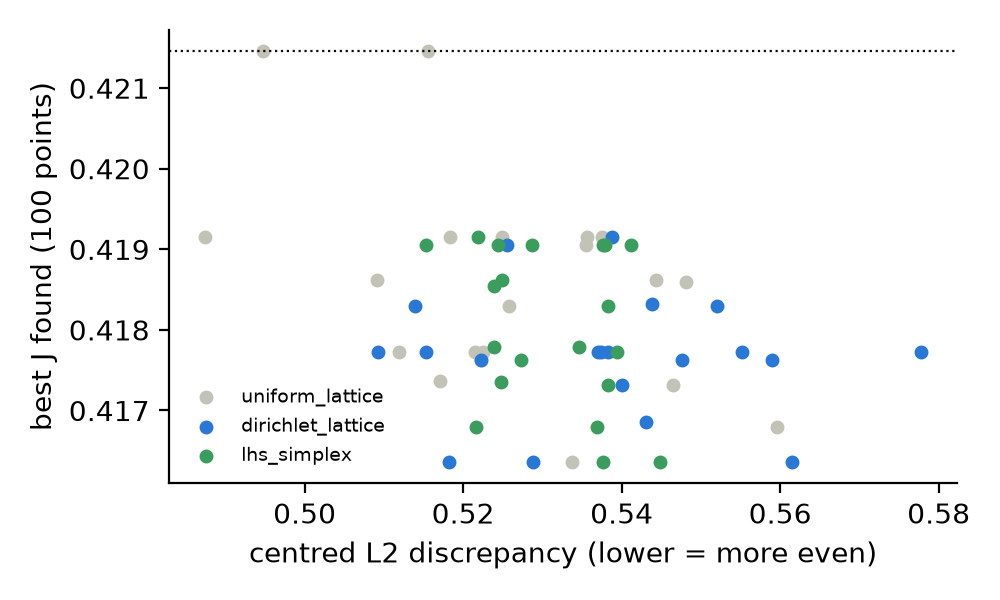
\includegraphics[width=0.8\textwidth]{fig_designs.png}
\caption{Any 100-point design finds the plateau; regret against the exhaustive optimum is at most 0.005.}
\label{fig:designs}
\end{figure}

\subsection{The optimum does not transfer, and neither does the rank}
Leave-one-dataset-out: weights re-fitted without the held-out dataset predict its ranking with mean $\tau=+0.34$, the full-data best with $+0.39$, v1 with $+0.37$ (Table~\ref{tab:lofo} gives the family-level version). Per-family optima pull in different directions (Figure~\ref{fig:family}): decay-dominated for EM and SM, recall-dominated for TQA, precision-heavy for FIN, yet none is far from the plateau. Changing only the pooling rule inside the objective moves v1's rank from 393 (Bradley--Terry) to 1,506 (Kemeny) and changes which weighting is ``best'', so rank inside a flat objective carries no information.

\begin{table}[htbp]
\centering\small
\caption{Leave-one-family-out. $\tau$ = agreement of the held-out family's pooled ranking with the pooled ranking of the remaining families.}
\label{tab:lofo}
\begin{tabular}{llccc}
\toprule
Held-out family & LOFO weights (F1 / decay / prec / rec) & $\tau$: LOFO weights & full best & v1 \\
\midrule
EM  (11 sets) & 0.20 / 0.00 / 0.50 / 0.30 & $+0.32$ & $+0.29$ & $+0.30$ \\
SM  (6 sets)  & 0.00 / 0.10 / 0.00 / 0.90 & $+0.35$ & $+0.37$ & $+0.25$ \\
TQA (11 sets) & 0.45 / 0.00 / 0.40 / 0.15 & $+0.38$ & $+0.40$ & $+0.38$ \\
FIN (3 sets)  & 0.00 / 0.95 / 0.05 / 0.00 & $+0.43$ & $+0.51$ & $+0.51$ \\
\bottomrule
\end{tabular}
\end{table}

\begin{figure}[htbp]
\centering
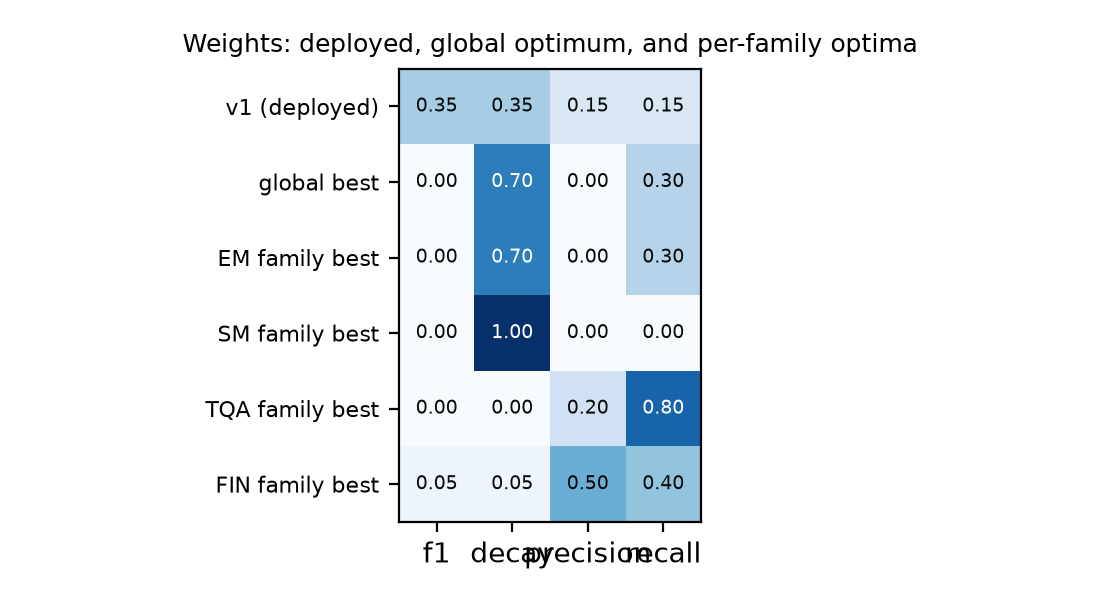
\includegraphics[width=0.85\textwidth]{fig_family_weights.png}
\caption{Deployed weights (v1), the global optimum and the per-family optima.}
\label{fig:family}
\end{figure}

\subsection{Agreement and correctness do not pull the same way}
On 31,380 synthetic answers of known utility, v1 scores $\rho=0.878$; the best weighting by $\rho$ reaches 0.883 and the best by $J$ only 0.845; exact match 0.828. Every rule separates correct from wrong answers with AUC 0.994. Across the lattice $J$ and $\rho$ correlate $-0.34$ on this cache and $+0.38$ on the previous one, which is what a flat $J$ predicts. The Pareto knee (F1 0.05, decay 0.60, precision 0.25, recall 0.10) is within 0.002 of the best $J$ and within 0.006 of the best $\rho$ (Table~\ref{tab:anchors}, Figure~\ref{fig:pareto}).

\begin{table}[htbp]
\centering\scriptsize
\setlength{\tabcolsep}{4pt}
\caption{Correctness on known-quality anchors (9,881 correct, 7,430 wrong, remainder partial). $\rho_d$ = mean per-dataset $\rho$; wrong = mean score given to wrong answers.}
\label{tab:anchors}
\begin{tabular}{llcccccc}
\toprule
Rule & F1 / decay / prec / rec & $J$ & $\rho$ & $\rho_d$ & AUC & wrong & hedge gap \\
\midrule
v1            & 0.35 / 0.35 / 0.15 / 0.15 & 0.404 & 0.878 & 0.868 & 0.994 & 0.034 & $-0.51$ \\
best $J$      & 0.00 / 0.70 / 0.00 / 0.30 & 0.421 & 0.845 & 0.840 & 0.994 & 0.037 & $-0.49$ \\
best $\rho$   & 0.00 / 0.35 / 0.60 / 0.05 & 0.398 & 0.883 & 0.871 & 0.994 & 0.034 & $-0.57$ \\
Pareto knee   & 0.05 / 0.60 / 0.25 / 0.10 & 0.419 & 0.877 & 0.866 & 0.994 & 0.036 & $-0.55$ \\
exact match   & --                        & --    & 0.828 & 0.830 & 0.989 & 0.011 & $-0.81$ \\
\bottomrule
\end{tabular}
\end{table}

\begin{figure}[htbp]
\centering
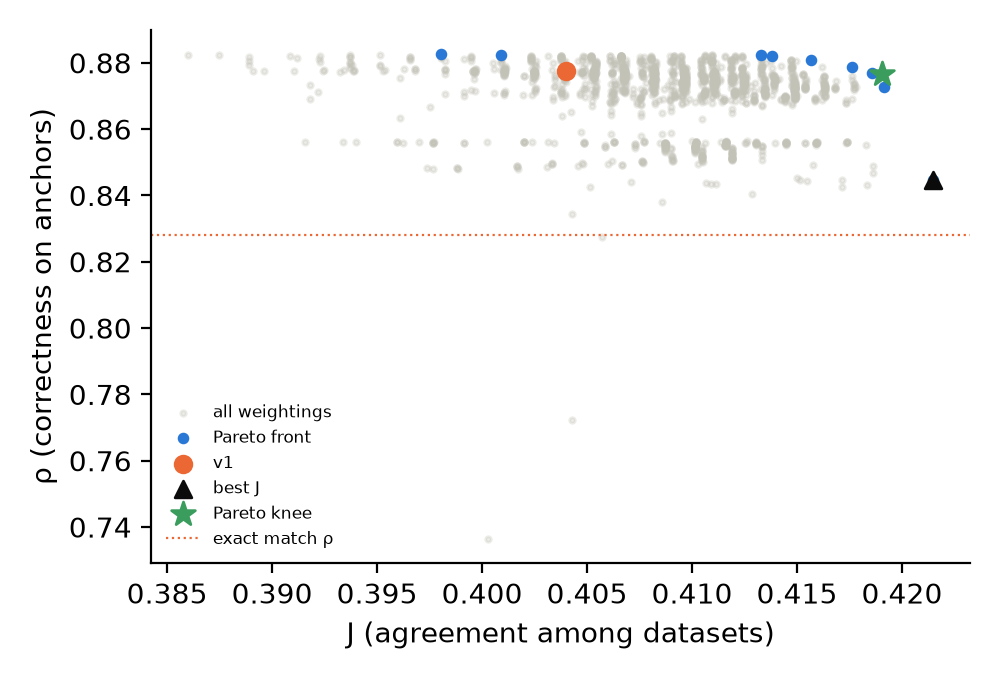
\includegraphics[width=0.75\textwidth]{fig_pareto.png}
\caption{Agreement $J$ against anchor correctness $\rho$ for every weighting; v1, the best-$J$, best-$\rho$ and knee points marked.}
\label{fig:pareto}
\end{figure}

\subsection{Leaderboard}
Under every rule the Friedman test rejects equal models ($p<0.001$) while datasets agree only moderately (Kendall's $W$ 0.26--0.28). The ends of the ranking are stable: Llama 3.3 70B is last and gpt-oss-120b ninth under every rule and every pooling method, with Holm-corrected significance against the top group. The order inside the top three depends on the rule and the pooling method (Table~\ref{tab:lb_v1}, Table~\ref{tab:lb_rules}, Figure~\ref{fig:leaderboard}): Bradley--Terry puts Gemini 3.8 Flash first under v1 and all calibrated rules, Borda puts GPT-5.5 first under v1 and Opus first under the top-5 rules, and exact match puts Opus first under both.

\begin{table}[htbp]
\centering\small
\caption{Leaderboard under the deployed rule (v1 weights). Bradley--Terry strength $\pm$ SE relative to Opus; Borda rank with 95\,\% bootstrap interval; mean composite score over the suite.}
\label{tab:lb_v1}
\begin{tabular}{llccc}
\toprule
Rank & Model & BT strength & Borda rank [95\,\%] & mean score \\
\midrule
1 & Gemini 3.8 Flash & $+0.12 \pm 0.02$ & 3 [1, 3] & 0.812 \\
2 & Claude Opus 5    & $+0.10 \pm 0.00$ & 2 [1, 3] & 0.811 \\
3 & GPT-5.5          & $+0.05 \pm 0.02$ & 1 [1, 3] & 0.808 \\
4 & Claude Sonnet 5  & $+0.03 \pm 0.02$ & 4 [4, 6] & 0.795 \\
5 & Grok 4           & $+0.03 \pm 0.02$ & 5 [4, 6] & 0.797 \\
6 & GPT-5.4-mini     & $-0.01 \pm 0.02$ & 8 [5, 8] & 0.789 \\
7 & DeepSeek-chat    & $-0.02 \pm 0.02$ & 7 [5, 8] & 0.783 \\
8 & DeepSeek-R1      & $-0.03 \pm 0.02$ & 6 [5, 8] & 0.788 \\
9 & gpt-oss-120b     & $-0.10 \pm 0.02$ & 9 [9, 10] & 0.767 \\
10 & Llama 3.3 70B   & $-0.17 \pm 0.02$ & 10 [9, 10] & 0.739 \\
\bottomrule
\end{tabular}
\end{table}

\begin{table}[htbp]
\centering\scriptsize
\caption{Bradley--Terry rank (Borda rank in brackets) under each reported rule. top1--top5 = the five best weightings by $J$; best-$\rho$ = best by anchor correctness; knee = $(J,\rho)$ Pareto knee.}
\label{tab:lb_rules}
\setlength{\tabcolsep}{2.5pt}
\begin{tabular}{lcccccccccc}
\toprule
Rule & Opus 5 & Sonnet 5 & DS-chat & DS-R1 & Flash 3.8 & 5.4-mini & GPT-5.5 & gpt-oss & Grok 4 & Llama \\
\midrule
exact match & 1 (1) & 5 (4) & 8 (7) & 7 (6) & 3 (3) & 6 (8) & 2 (2) & 9 (9) & 4 (5) & 10 (10) \\
v1          & 2 (2) & 4 (4) & 7 (7) & 8 (6) & 1 (3) & 6 (8) & 3 (1) & 9 (9) & 5 (5) & 10 (10) \\
top1        & 2 (1) & 4 (4) & 7 (8) & 6 (6) & 1 (3) & 8 (7) & 3 (2) & 9 (9) & 5 (5) & 10 (10) \\
top2        & 2 (1) & 4 (4) & 6 (7) & 8 (6) & 1 (3) & 7 (8) & 3 (2) & 9 (9) & 5 (5) & 10 (10) \\
top3        & 2 (1) & 4 (4) & 6 (7) & 8 (6) & 1 (3) & 7 (8) & 3 (2) & 9 (9) & 5 (5) & 10 (10) \\
top4        & 2 (1) & 4 (4) & 7 (8) & 8 (6) & 1 (3) & 6 (7) & 3 (2) & 9 (9) & 5 (5) & 10 (10) \\
top5        & 2 (1) & 4 (4) & 7 (8) & 6 (6) & 1 (3) & 8 (7) & 3 (2) & 9 (9) & 5 (5) & 10 (10) \\
best-$\rho$ & 2 (2) & 4 (4) & 8 (8) & 7 (6) & 1 (3) & 5 (7) & 3 (1) & 9 (9) & 6 (5) & 10 (10) \\
knee        & 2 (1) & 4 (4) & 7 (8) & 8 (6) & 1 (3) & 6 (7) & 3 (2) & 9 (9) & 5 (5) & 10 (10) \\
\midrule
\multicolumn{11}{l}{Kendall $\tau$ between the BT rankings of the rules: 0.78--1.00 (exact match vs the rest 0.78--0.82).} \\
\bottomrule
\end{tabular}
\end{table}

\begin{figure}[htbp]
\centering
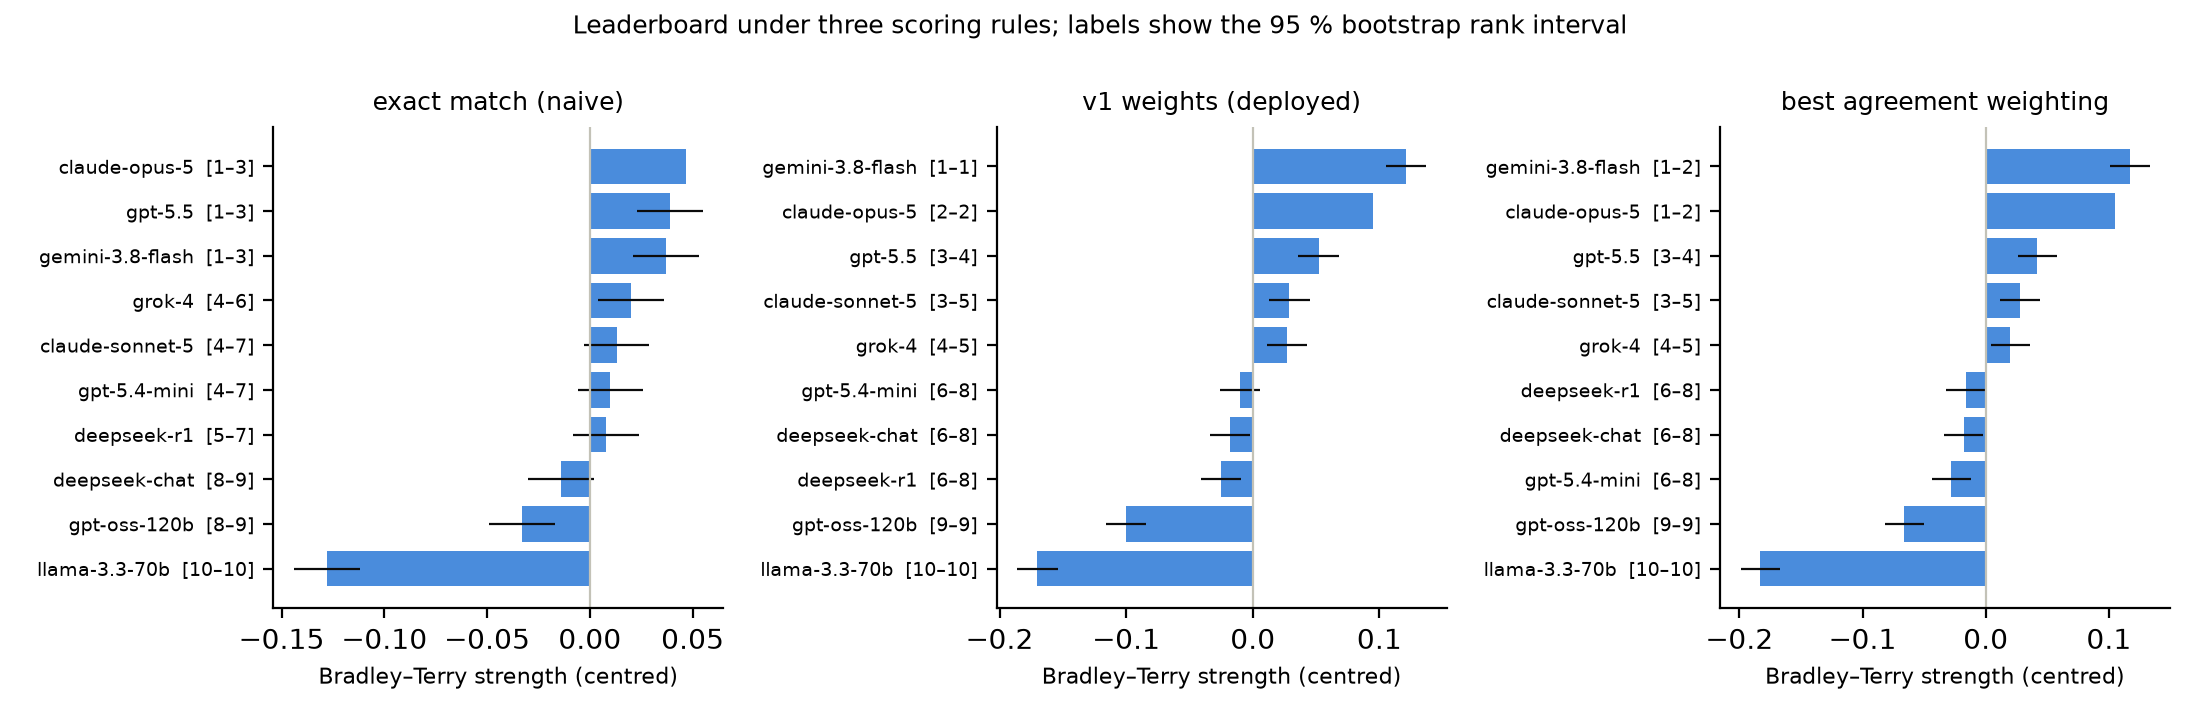
\includegraphics[width=0.95\textwidth]{fig_leaderboard_rules.png}
\caption{Bradley--Terry strengths $\pm$ SE with bootstrap rank intervals under exact match, v1 and the best-$J$ weighting. The ends are stable; the top order is rule-dependent.}
\label{fig:leaderboard}
\end{figure}

\begin{figure}[htbp]
\centering
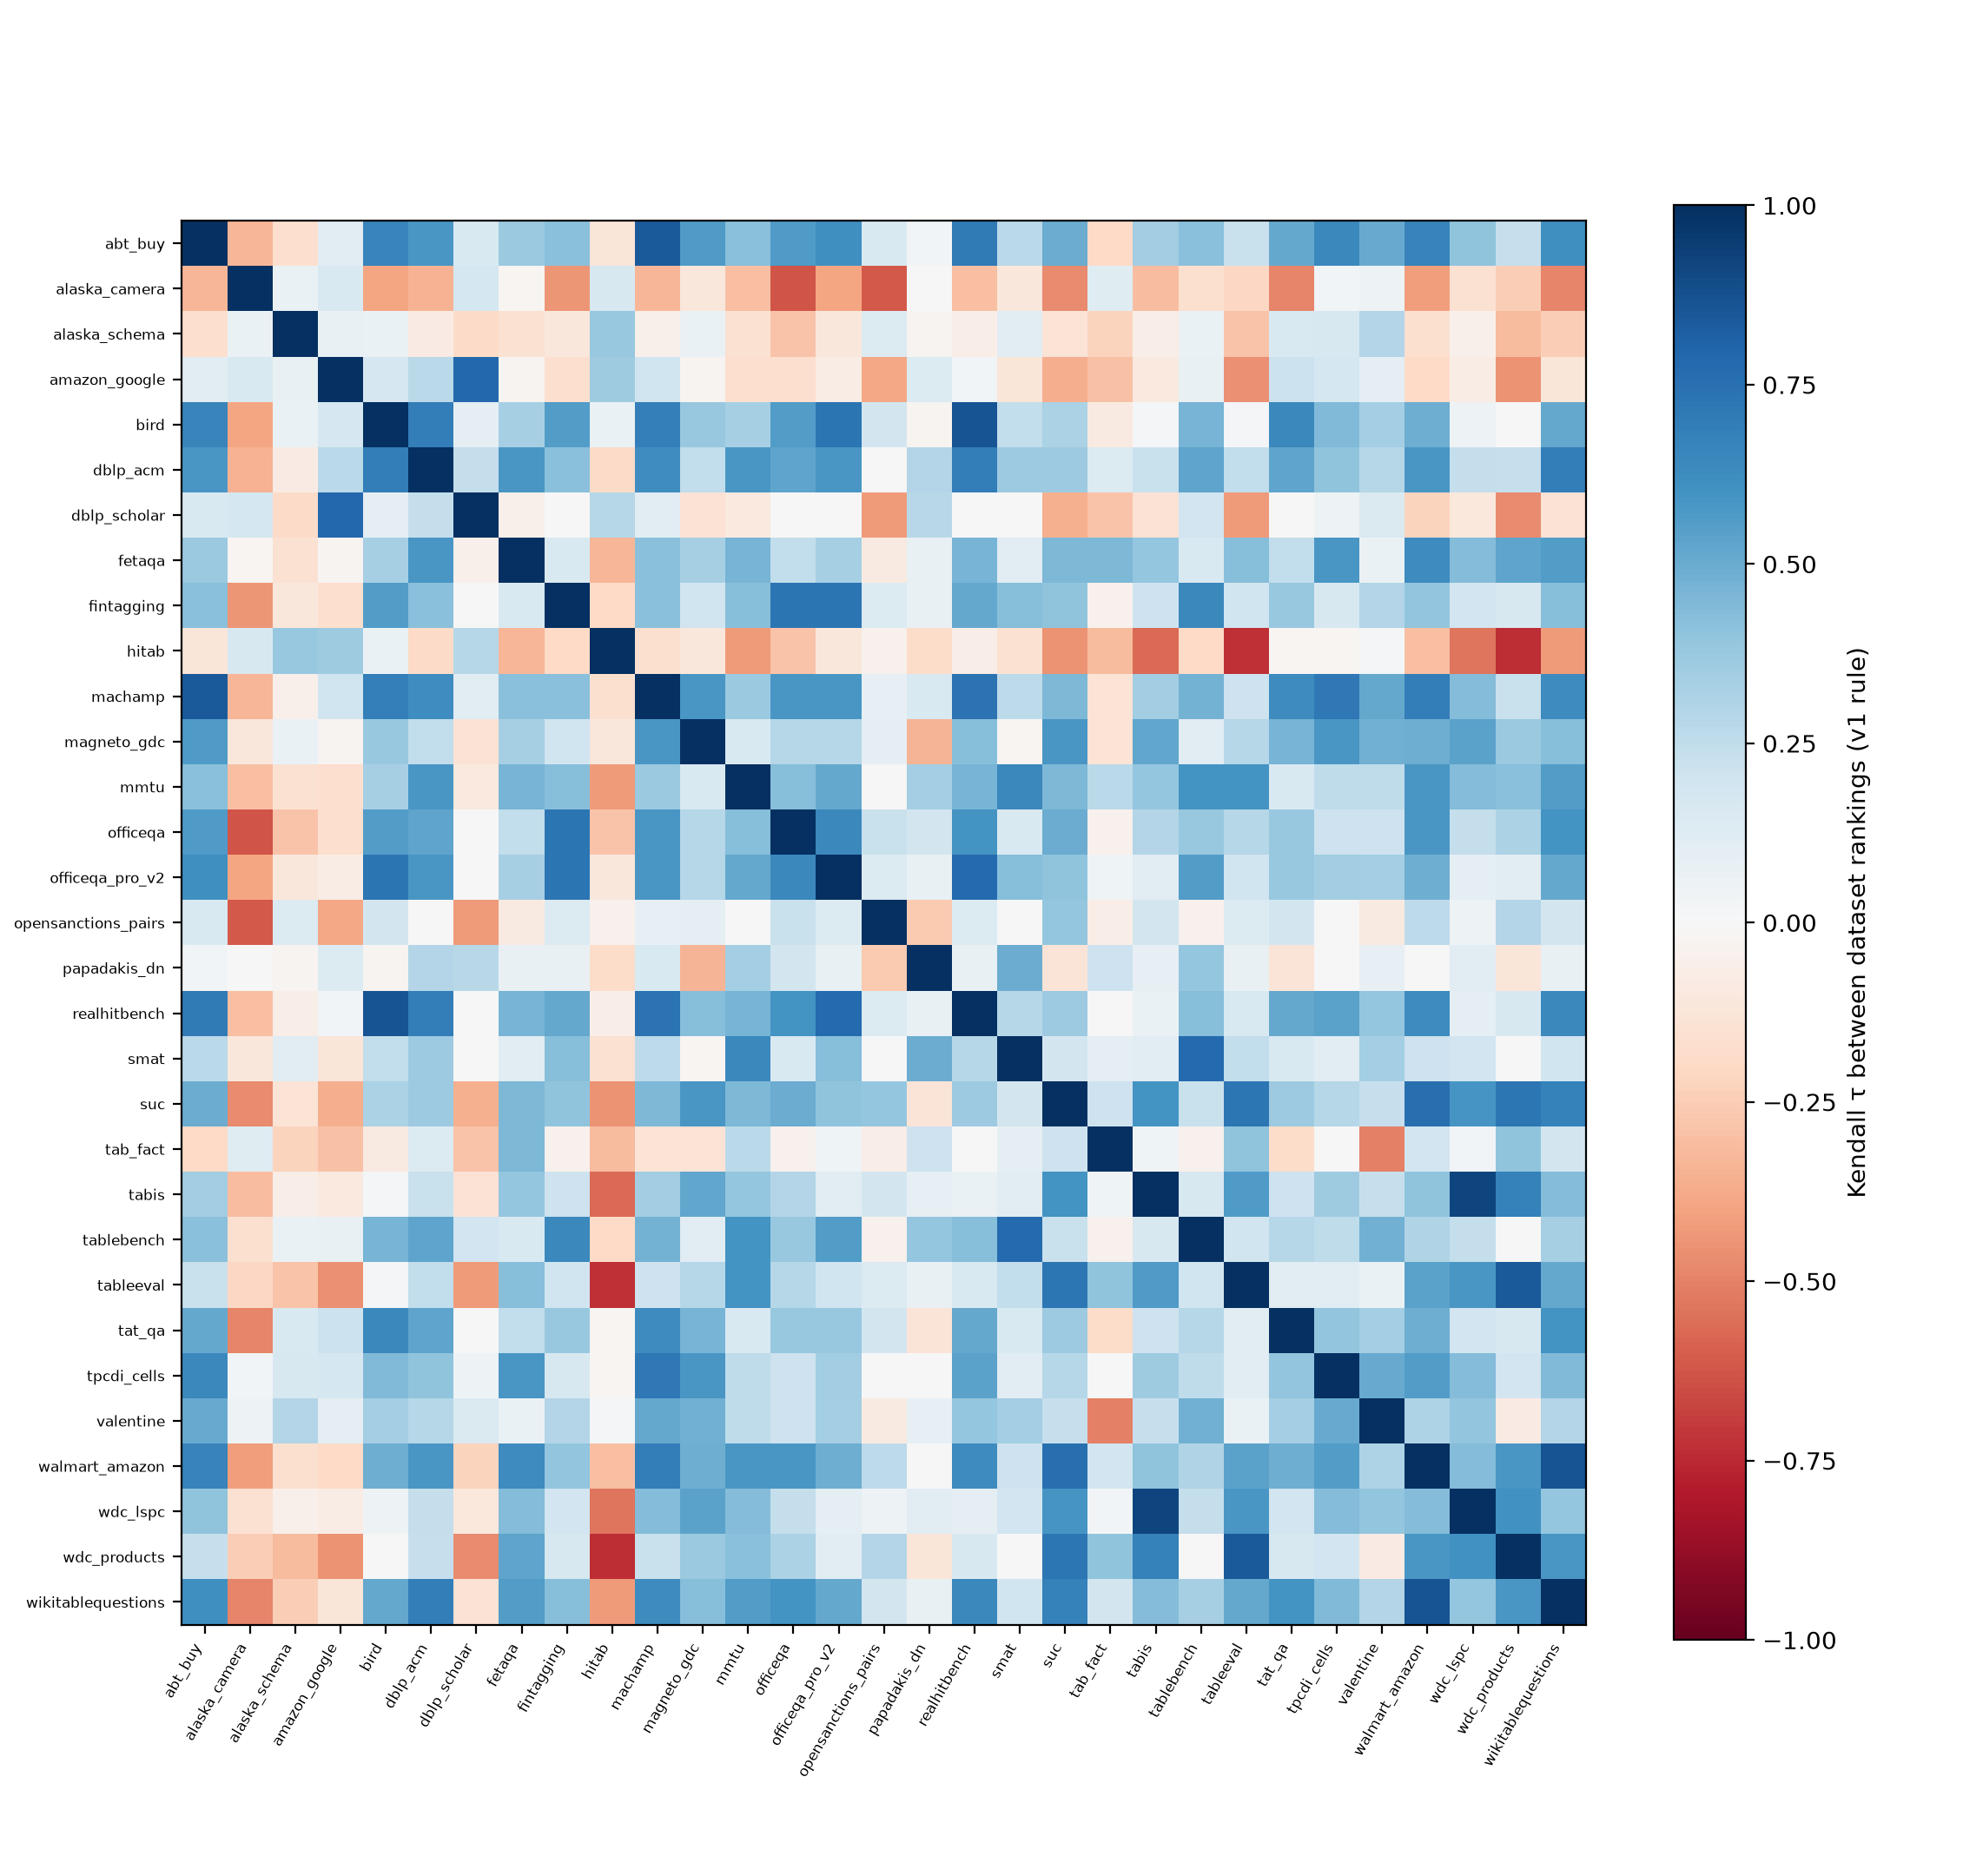
\includegraphics[width=0.8\textwidth]{fig_dataset_tau.png}
\caption{Kendall $\tau$ between the model rankings of each pair of datasets under v1. Datasets agree only moderately ($W\approx0.27$).}
\label{fig:dataset_tau}
\end{figure}

\subsection{Comparability with published numbers}
Post-stratification to the official split changes dataset accuracy by at most 0.09 (OpenSanctions pairs 0.82 $\to$ 0.73; TAT-QA 0.80 $\to$ 0.76; MMTU 0.87 $\to$ 0.83). For the matching sets, positive-class F1 computed on the balanced 50/50 pool overstates F1 at the official match ratio wherever the official split is sparse (Table~\ref{tab:official}, Figure~\ref{fig:official}).

\begin{table}[htbp]
\centering\small
\caption{Matching sets under v1, averaged over the ten models: suite accuracy, post-stratified official accuracy, and positive-class F1 on the balanced pool vs at the official match ratio.}
\label{tab:official}
\begin{tabular}{lccccc}
\toprule
Dataset & official match share & suite acc. & official acc. & F1 (pool) & F1 (official ratio) \\
\midrule
Abt--Buy           & 0.108 & 0.970 & 0.986 & 0.968 & 0.936 \\
Amazon--Google     & 0.102 & 0.936 & 0.932 & 0.929 & 0.739 \\
Walmart--Amazon    & 0.094 & 0.958 & 0.975 & 0.947 & 0.875 \\
DBLP--ACM          & 0.180 & 0.986 & 0.991 & 0.985 & 0.976 \\
DBLP--Scholar      & 0.186 & 0.949 & 0.966 & 0.948 & 0.910 \\
WDC Products 2024  & 0.280 & 0.978 & 0.985 & 0.979 & 0.974 \\
WDC LSPC 2017      & 0.264 & 0.982 & 0.983 & 0.983 & 0.971 \\
Machamp            & 0.175 & 0.887 & 0.890 & 0.892 & 0.733 \\
Papadakis--Christen Dn & 0.018 & 0.941 & 0.988 & 0.833 & 0.683 \\
OpenSanctions pairs & 0.769 & 0.821 & 0.727 & 0.773 & 0.777 \\
Alaska Camera      & n/c   & 0.958 & --    & 0.955 & -- \\
\bottomrule
\end{tabular}
\end{table}

\begin{figure}[htbp]
\centering
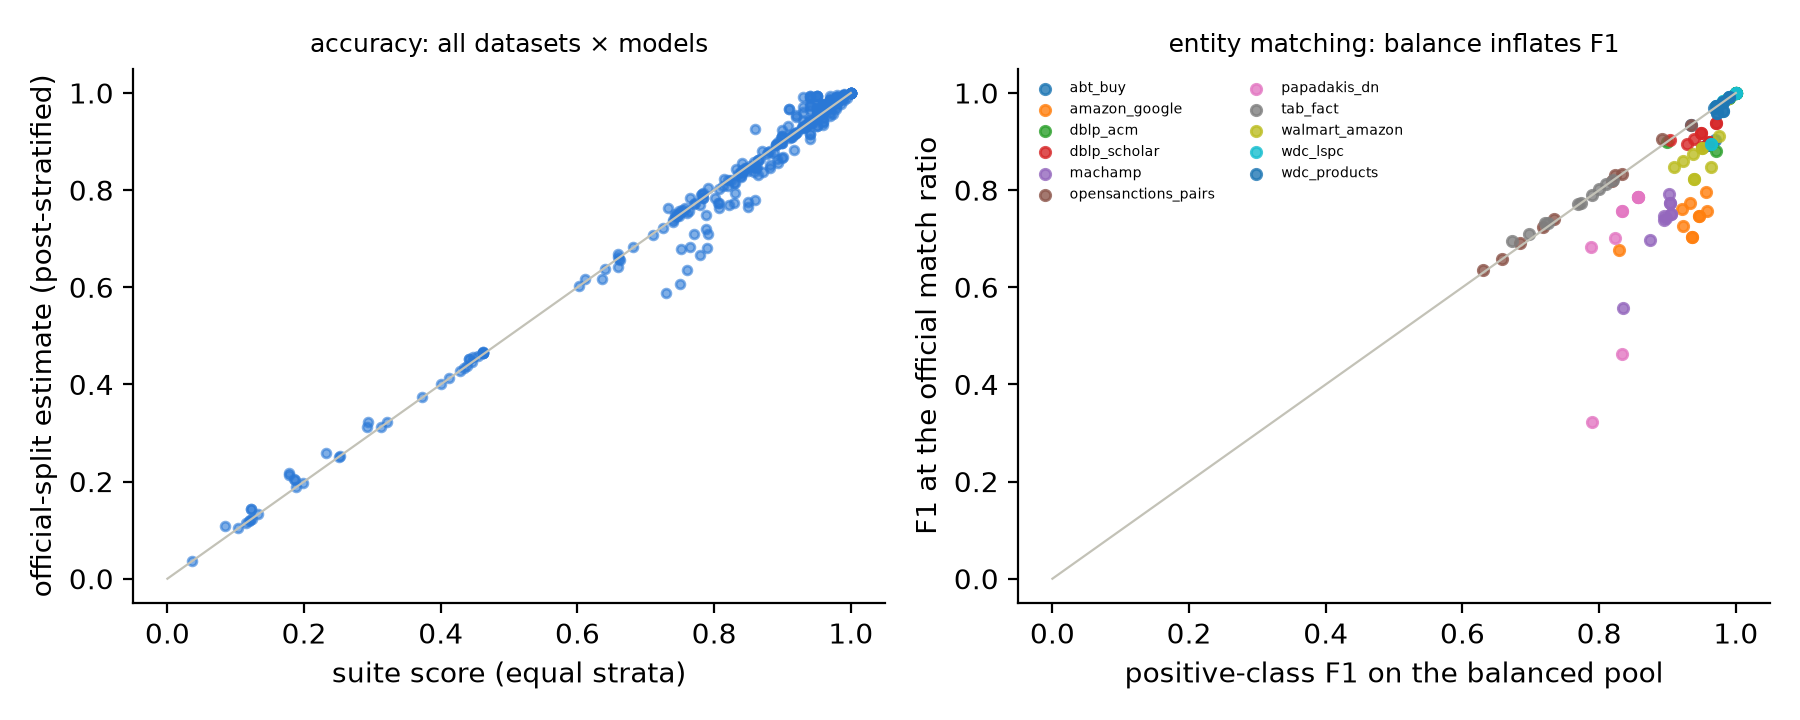
\includegraphics[width=0.9\textwidth]{fig_official_split.png}
\caption{Suite score vs post-stratified official estimate per dataset, and matching F1 on the balanced pool vs at the official match ratio.}
\label{fig:official}
\end{figure}

\subsection{Dataset diagnostics}
Three datasets sit at ceiling (mean composite 0.98 with a spread of 0.02--0.04 across models): Valentine, WDC LSPC and WDC Products. They are flagged and remain inside the objective in this run. Two sit near floor for every model (OfficeQA closed-book 0.13, OfficeQA Pro V2 0.14) and one is a known hard set (BIRD 0.19); none is excluded. Self-stability $\tau$ (rank agreement between split halves of a dataset) ranges from 0.58 (HiTab) to 0.93 (FeTaQA).

% =====================================================================
\section{Some shortcomings / finalisations}
% (user text, unchanged)
\begin{itemize}
\item Limitations ran into:
\begin{itemize}
\item Tried Temperature = 0 for perfect reproducibility on output; Claude 5 and GPT-5.5 rejected.
\item Ran into some non-terminating answers (over token usage bounds set of 700 tokens, categorised as no-match / false value), tested via rerunning, total amount halved, and is negligible but still a notable edge-case.
\item Need human-labelling to account for proper ``human preference'' claims (from Chatbot Arena).
\item Need to rerun Gemini 3.0 Pro model (token usage messed up writing into results).
\item USD 161 for the ten models (Opus 99).
\end{itemize}
\end{itemize}

% =====================================================================
\appendix
\section{Dataset-specific format transformations and pipelining}
% (user text, unchanged; not part of the written eval)

\subsection*{Process of taking data from each dataset}
\begin{enumerate}
\item Official splits only, taken from the original papers; conducted a random sample (seeded) for finding 150 elements.
\item Prompted each model on each of 100 initial prompts to get model answers (accounted for aliases and unit handling).
\item Used native dataset-specific metrics as baseline from the 100 prompts' ground-truth golds.
\end{enumerate}

\subsection*{Entity matching (pair $\to$ yes/no; exact match native; official-ratio F1 by post-stratification)}
\begin{itemize}
\item Abt-Buy, Amazon-Google, Walmart-Amazon, DBLP-Scholar, DBLP-ACM --- Mudgal et al.\ 2018. Official test pairs; balanced 50/50 sample of 150; records as attribute lines.
\item WDC Products 2024 --- Peeters, Der \& Bizer 2024. Hard-negative test split; balanced per product category.
\item WDC LSPC 2017 --- Li et al.\ 2020 (Ditto). Four category test sets; balanced per category; pairs already in WDC Products excluded.
\item Machamp --- Wang et al.\ 2021. Seven heterogeneous-schema tasks; balanced within each task.
\item Papadakis--Christen Dn1--Dn8 --- Papadakis et al.\ 2024. Uniform sampling within each set, real class ratio kept (1.8 percent); the only unbalanced matching set.
\item Alaska Camera --- Crescenzi et al.\ 2021. Pairs built from the contest's entity clusters with hard negatives; not comparable to a published split.
\item OpenSanctions pairs --- dataset card. Its own 1,000-pair sample; balanced; non-commercial licence.
\end{itemize}

\subsection*{Schema matching (one question per source column; exact match native)}
\begin{itemize}
\item Valentine --- Koutras et al.\ 2021. Four table pairs per sub-benchmark and pair type; candidates trimmed but always containing the gold; full gold mapping stored for set-level F1.
\item Magneto GDC --- Liu et al.\ 2025. 40 of 736 targets shown; many-to-one golds as aliases.
\item SMAT --- Zhang et al.\ 2021. True target plus nine hard negatives from the same OMOP table.
\item Alaska schema --- Crescenzi et al.\ 2021. Monitor half only (93 items); attribute plus three sample values plus target list.
\item FinTagging --- 2025. Concept-linking task only; ten candidate XBRL concepts; half text, half table.
\item TPC-DI cells --- TPC 2014. The benchmark's own join-and-aggregate task, one item per customer cell.
\end{itemize}

\subsection*{Table QA and understanding}
\begin{itemize}
\item WikiTableQuestions --- Pasupat \& Liang 2015. Official test; typed golds with aliases.
\item TabFact --- Chen et al.\ 2020. Official test; entailed/refuted as yes/no.
\item FeTaQA --- Nan et al.\ 2022. Free-form gold; ROUGE-L native.
\item HiTab --- Cheng et al.\ 2022. Official test; number/text golds.
\item MMTU --- 2025. Nine of 25 tasks with short golds; task as stratum.
\item RealHiTBench --- 2025. Fact-checking and numerical questions only; tables capped; list golds.
\item SUC --- Sui et al.\ 2024. Six structural tasks regenerated from the source tables.
\item TabIS --- 2024. Zero-shot; option letter with text alias.
\item TableEval --- 2025. Eight short-gold sub-tasks; original instructions kept.
\item TableBench --- Wu et al.\ 2025. Two sub-types; numeric and list golds.
\item BIRD --- Li et al.\ 2023. Gold SQL executed by us; result value is the gold; schema plus evidence in context.
\end{itemize}

\subsection*{Financial documents}
\begin{itemize}
\item TAT-QA --- Zhu et al.\ 2021. Official dev; answers stratified by form; unit and scale handling.
\item OfficeQA Pro V2 --- 2026 dataset card. All 90 questions; referenced pages in context under a 6,000-character budget.
\item OfficeQA closed-book --- the original set; kept for continuity, every model at floor, excluded from the objective.
\end{itemize}

\end{document}
